%% COMPX523-26A Assignment 3 — Anti-Bunching Copilot
%% Restyled to the report template (article class); author--year refs via natbib.

\documentclass[11pt,a4paper]{article}

% ---------- Packages ----------
\usepackage[utf8]{inputenc}
\usepackage[T1]{fontenc}
\usepackage{lmodern}
\usepackage[margin=2.3cm]{geometry}
\usepackage{microtype}
\usepackage{graphicx}
\usepackage{booktabs}
\usepackage{array}
\newcolumntype{P}[1]{>{\centering\arraybackslash}p{#1}}
\usepackage{tabularx}
\usepackage{longtable}
\usepackage{multirow}
\usepackage{caption}
\usepackage{subcaption}
\usepackage{float}
\usepackage{amsmath}
\usepackage{amssymb}
\usepackage{textcomp}
\usepackage[table]{xcolor}
\usepackage{listings}
\usepackage{enumitem}
\usepackage{url}
\usepackage{tikz}
\usetikzlibrary{arrows.meta, positioning, shapes.geometric, decorations.pathreplacing}
\usepackage[ruled,vlined]{algorithm2e}
\usepackage[round,authoryear]{natbib}
\usepackage[hidelinks]{hyperref}  %% clickable citations, cross-refs, and DOIs (load last)

% ---------- Listings (code block styling) ----------
\definecolor{codebg}{RGB}{248,248,248}
\definecolor{codecomment}{RGB}{106,153,85}
\definecolor{codestring}{RGB}{163,21,21}
\definecolor{codekey}{RGB}{0,0,180}
\lstset{
  basicstyle=\ttfamily\footnotesize,
  backgroundcolor=\color{codebg},
  commentstyle=\color{codecomment},
  stringstyle=\color{codestring},
  keywordstyle=\color{codekey},
  language=Python,
  showstringspaces=false,
  breaklines=true,
  frame=single,
  framesep=4pt,
  rulecolor=\color{black!20},
  columns=fullflexible,
}

% ---------- Misc ----------
\newcommand{\code}[1]{\texttt{#1}}
\renewcommand{\arraystretch}{1.15}
\setlist{itemsep=2pt, topsep=2pt}

% ---------- Title metadata ----------
\title{An Online Anti-Bunching Copilot for Bus Drivers:\\
Streaming Headway-Risk Prediction on the SUNT Dataset}
\author{Ademar Tutor, Zaimei Xing, Member~3, Member~4, Member~5, Member~6 \\
\small Department of Computer Science, University of Waikato, Hamilton, New Zealand \\
\small COMPX523-26A: Machine Learning for Data Streams}
\date{}

\begin{document}
\maketitle

% ---------- Abstract ----------
\begin{abstract}
Bus bunching is the classic instability of high-frequency transit. A late bus collects
more passengers, slows further, and is caught by the following bus. The result is long
waits and uneven crowding. We propose a driver-facing
\emph{anti-bunching copilot}: an online (streaming) model that predicts, in real time,
when a bus is about to bunch with the bus ahead and nudges the individual driver to ease
off. The intervention is advisory and needs no new infrastructure or central control room.
Using the per-vehicle \emph{Origin--Destination} (OD) records of the Salvador Urban Network
Transportation (SUNT) dataset, we reconstruct per-bus trajectories, compute the
\emph{forward headway} to the bus ahead, and frame the task as online classification of
next-window bunching risk. We replay the data as a chronological stream and evaluate
prequentially (test-then-train) with imbalance-aware metrics. We first show, descriptively,
that the problem is real: across the eight busiest routes the within-hour headway coefficient
of variation is $0.80$ and irregular spacing imposes on the order of half a million avoidable
passenger-waiting-minutes per day. In a bake-off of CapyMOA learners on these routes
(109{,}029 instances), an Adaptive Random Forest (ARF) attains the best bunching-class F1
(0.916) and balanced accuracy (0.915), and --- unlike the non-learning baselines --- fires its
warning a median of $\approx$28 minutes before the observed bunching, which is the property
that makes a driver nudge actionable. A clearly-labelled counterfactual simulation, in which
nudged drivers ease off by a few seconds, estimates a $\approx$13\% reduction in bunching
events and a $\approx$10\% reduction in excess waiting --- an effect that is a simulation under
stated assumptions, not a measured field outcome.
\end{abstract}

\medskip
\noindent\textbf{Keywords:} bus bunching; data stream mining; concept drift; ADWIN;
Adaptive Random Forest; prequential evaluation; SUNT; Salvador

\clearpage

%% ======================================================================
\section{Introduction}
\label{sec:intro}

Many people in Salvador, Brazil depend on public transport, and most of them travel by bus
\citep{bndes2025salvador, Ferreira2025}. The city also has heavy road traffic, and is one of the more
congested cities in the world \citep{tomtom2025salvador, tomtom2025ranking}. Large transport projects
are difficult to deliver here, because responsibility is split across many public and private bodies
and the bus system is under serious financial strain \citep{tcebahia2022compensacao,
worldbank2026salvador}. These conditions favour interventions that work with the buses and data that
already exist, cost little, and do not rely on agencies coordinating with each other. We therefore
study service reliability using the Salvador Urban Network Transportation (SUNT) dataset
\citep{Ferreira2025}, and let what is realistic to deploy in this setting, not only what is
technically possible, shape the design.

Within these constraints, we do not build a planner-facing dashboard, which mostly tells an
authority something it would still need budget and political will to act on. Instead we target the
one actor who can act \emph{immediately} and at zero cost: the individual driver. The failure that
driver can address is \emph{bus bunching}. Headway-based services are unstable by nature: a small
delay snowballs, because a late bus collects the passengers an on-time bus would have carried, which
slows it further, while the bus behind finds fewer passengers, speeds up, and closes the gap. The
result is one of the most common service-quality failures in urban transit. Because it can be
mitigated behaviourally, by a driver easing off or briefly holding, our intervention is advisory and
needs no new infrastructure.

Figure~\ref{fig:bunching} contrasts the intended evenly-spaced service with the bunched
state \citep{Enayatollahi2019}: in the top row, five buses are 15~minutes apart; in the
bottom row, four buses have collapsed into a platoon one minute apart while the lead bus
has pulled 57~minutes ahead, leaving an overcrowded front bus followed by near-empty ones.
For clarity, we use the following terms throughout the report:

\begin{itemize}
\item \textbf{Headway:} the time gap between successive buses arriving at the same stop.
  Even headways are the goal of high-frequency service.
\item \textbf{Bus bunching:} the unstable state in which buses that should be evenly spaced
  clump into a platoon, leaving a large gap behind them (Figure~\ref{fig:bunching}, bottom).
\item \textbf{Dwell time:} the time a bus spends stopped to board and alight passengers.
  Heavy boarding lengthens dwell, which is a primary driver of bunching.
\item \textbf{Forward headway:} the gap from a given bus to the bus \emph{ahead} of it on the
  same route. This is the core signal our model predicts.
\item \textbf{OD data:} the per-vehicle Origin--Destination records of SUNT, where each row is
  one bus arriving at one stop with its exact arrival time and onboard load.
\item \textbf{Driver nudge:} the system's advisory output to the driver, namely ``ease off /
  let the gap open'' or ``hold briefly at this stop''. It never asks the driver to speed up.
\item \textbf{Bunching-risk classes:} the three-way label the model predicts for the next
  window, \{ok, warning, bunching\}.
\item \textbf{Nudge lead time:} how many minutes before an observed bunching event the warning
  fires. A warning is only useful if it arrives early enough for the driver to act.
\end{itemize}

\begin{figure}[htbp]
\centering
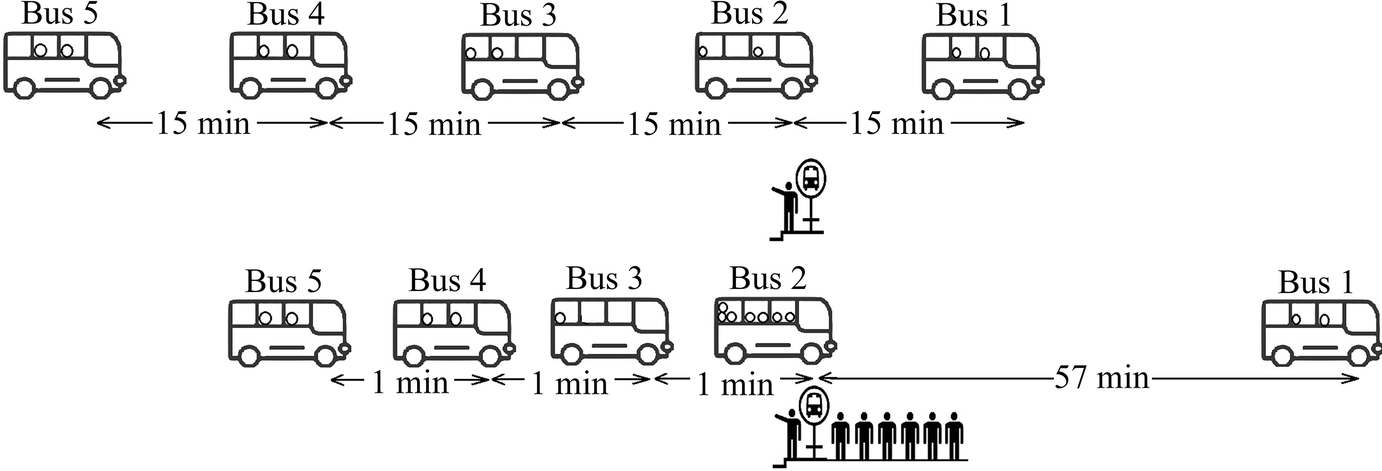
\includegraphics[width=\linewidth]{figures/12469_2019_203_Fig1_HTML.png}
\caption{Evenly-spaced service (top) versus bunched service (bottom). When a bus runs late,
the growing gap ahead of it lets passengers accumulate; the longer it dwells to board them,
the later it gets, while the bus behind catches up. Adapted from \citet{Enayatollahi2019}.}
\label{fig:bunching}
\end{figure}

This feasibility constraint also dictates the data we can use. Bunching is defined on the
\emph{headway} between two \emph{successive} buses, which can only be measured if each bus is
identified individually and its arrivals are ordered in time. The aggregated 5- and 30-minute
tables provided with the assignment store only per-interval \emph{counts}, with no individual
vehicle identifier, trip identifier, or exact arrival time. As a result, when two buses pass a stop
within the same window, the data cannot distinguish a 30-second gap (bunched) from a four-minute gap
(normal). The aggregation removes the very signal the task depends on. We therefore use the raw
\emph{Origin--Destination} (OD) records from the same published SUNT release, which retain
per-vehicle arrivals with exact stop times and make headways directly computable; the assignment
brief explicitly encourages additional public data. We set out this schema-level argument and a
side-by-side comparison of the two data products in Section~\ref{sec:data} (Table~\ref{tab:schema}).

The problem is also a genuine \emph{machine-learning-for-data-streams} task. Headway dynamics
are non-stationary: they change with time of day, demand, traffic, weather, and network
changes. A static model or fixed rule mis-fires after any shift. Online learning with
\emph{prequential} evaluation, strict chronological ordering, and drift adaptation
\citep{Bifet2007} is the appropriate tool, and the per-bus stream is naturally replayed from
SUNT by timestamp. A small in-cab prototype could surface the model's output as a glanceable
risk light and a short nudge. In what follows we (i) establish descriptively that bunching is a
real and costly problem on these routes, (ii) bake off CapyMOA learners under prequential
evaluation to find one that warns early enough to act on, and (iii) estimate the plausible effect
of a small, bounded driver ease-off in a clearly-labelled counterfactual simulation.

%% ======================================================================
\section{Related Work}
\label{sec:related}

This work sits at the intersection of transit operations and machine learning for data streams, and
we position it along three lines. We first place bunching in its wider operational context, namely how
bus operations and bunching interact with road traffic (Section~\ref{sec:rw-traffic}). We then review
how prior work predicts and controls bunching, and where those approaches assume infrastructure or
central authority that the Salvador setting lacks (Section~\ref{sec:rw-bunching}). Finally we turn to
the data-stream learning methods this study adapts to the problem (Section~\ref{sec:rw-ml}). Across
all three, the gap we address is the same: prior work tends to act centrally or offline, whereas we
target a decentralised, online, per-driver nudge.

\subsection{Buses, bunching, and road traffic}
\label{sec:rw-traffic}
Bus operations interact with the surrounding road traffic. This matters for an intervention that
adjusts a bus's pace. \citet{NguyenPhuoc2018} estimate the \emph{net} effect of bus operations on
network congestion and find it positive overall. In Melbourne, buses cut severely congested links by
roughly a tenth by keeping would-be drivers off the road. At the same time, the congestion \emph{cost}
of buses is concentrated at stops, where stop-start dwell reduces road capacity. This is relevant here
because dwell is also the mechanism that drives bunching. The same stop dynamics therefore underlie
both phenomena, and improving bus reliability may help protect the road-congestion benefit that buses
provide. A natural concern is that an intervention which deliberately delays a bus could worsen road
traffic. \citet{Qiang2023} address this concern with a cellular-automaton simulation of \emph{mixed}
traffic. They show that self-equalising headway control continues to regulate bus spacing on
non-dedicated lanes. It also does not appear to harm car speed or overall capacity, and at
intermediate density it may modestly improve them, though this evidence comes from an idealised
synthetic route rather than field data. Both studies treat the bus and traffic interaction with
offline planning or simulation models and with network- or fleet-level levers. This is useful for
bounding the wider congestion effects of bus operation. It leaves open the per-vehicle, real-time
setting that this study targets, in which the lever is a single driver's voluntary ease-off rather
than a centrally imposed policy.

\subsection{Predicting and controlling bus bunching}
\label{sec:rw-bunching}
Bunching and headway instability are long studied. \citet{Enayatollahi2019} characterise the
headway as intrinsically unstable and show that even a small reduction in per-passenger boarding
time, or limiting a delayed bus's dwell at stops, can markedly reduce bunching. Classical
\emph{control} schemes act by delaying a bus rather than speeding one up: \citet{Daganzo2009}
proposed adaptive holding/headway control that keeps spacing even, \citet{Bartholdi2012} make
headways \emph{self-equalising} by holding each arriving bus in proportion to the headway behind
it, and \citet{DaganzoPilachowski2011} achieve the same end through two-way speed cooperation, in
which a leading bus eases off for the one behind but is never asked to exceed its normal speed.
This ``slow the leader, never the follower'' principle is the action our advisory approximates. A
separate \emph{prediction} line forecasts bunching before it forms: \citet{Yu2016} predict
stop-level headway from smart-card data and flag over 95\% of events several stops ahead, and
\citet{BorgesSantos2022} predict bunching up to ten stops ahead with a tree ensemble on Brazilian
GPS/GTFS data. These predict but do not act, and \citet{MoreiraMatias2016} close the loop with an
online learning framework that detects and counters bunching in real time, reporting large
reductions in bunching and meaningful waiting-time savings. Most such schemes nonetheless assume a
\emph{central controller} issuing holds; our contribution is a driver-personal, decentralised
nudge driven by an online stream model, with no control room.

\subsection{Adapting machine learning for data streams to bus bunching}
\label{sec:rw-ml}
Predicting bunching online means treating each bus arrival as one event in an unbounded,
non-stationary stream, which calls for learners that update incrementally and adapt to change.
Hoeffding Trees learn decision trees incrementally from unbounded streams using the Hoeffding
bound to decide splits \citep{Domingos2000}. The adaptive variant couples the tree with
ADWIN-monitored branches that self-replace under drift \citep{Bifet2009}. Adaptive Random
Forest (ARF) extends streaming forests with online bagging, random feature subspaces, per-tree
drift detection, and weighted voting \citep{Gomes2017}. Because our positive class is rare and its
prevalence drifts across the day, the relevant subfield is learning from \emph{imbalanced} data
streams, which is now systematically benchmarked: \citet{Aguiar2024} compare 24 stream classifiers
across 515 imbalanced, drifting benchmarks and recommend reporting complementary, imbalance-aware
metrics rather than accuracy, while \citet{WangMinkuYao2015} give the canonical online-resampling
baselines (OOB/UOB) that re-tune sampling as the imbalance ratio shifts. We access these learners
through CapyMOA \citep{CapyMOA2024}, which exposes the MOA engine in Python with prequential
tooling. Underpinning these adaptive learners, ADWIN detects distribution change with an adaptive
window and guarantees \citep{Bifet2007}; we use it both inside the learners and as a drift log,
so the model tracks the time-of-day and demand shifts that bunching dynamics exhibit.

%% ======================================================================
\section{Methodology}
\label{sec:method}

Our central idea is to avert bunching before it forms, rather than reacting to it after the fact:
because a bunching event begins as a single bus drifting off its headway, it can be averted by a
small, timely adjustment from that one driver. Realising this idea has four requirements, and this
section addresses them in turn. We first establish what data the approach needs and why the chosen
source supplies it (Section~\ref{sec:data}), since the whole method is built on a quantity that the
data must let us measure. We then present the streaming driver-nudge system itself
(Section~\ref{sec:system}), the preprocessing that turns raw operational records into the stream the
model consumes (Section~\ref{sec:preprocessing}), and the counterfactual simulation used to estimate
the effect of acting on its predictions (Section~\ref{sec:simdesign}).

\subsection{Data requirements and source}
\label{sec:data}

The approach hinges on the \emph{headway}: the time gap between two \emph{successive} buses arriving
at the same stop, which is the quantity bunching is defined on. Before describing the system, we
therefore establish what data is needed to measure the headway, and why the source we use supplies it
while the data provided by the assignment does not.

To measure the headway, the data must let us identify each bus individually and order its
arrivals in time. Concretely, every record needs the individual vehicle, the individual trip, and
the exact arrival time at the stop. Without all three, successive buses cannot be told apart and
the gap between them cannot be computed (Table~\ref{tab:schema}).

The assignment supplies a 10-stop subset of SUNT in two pre-aggregated versions, at 5-minute and
30-minute resolution. These tables are keyed by (stop, time-interval) and store only per-interval
\emph{counts}, such as boardings, loading, and the number of vehicles. They carry no individual
vehicle identifier and no exact arrival timestamp. If two buses pass a stop within the same
5-minute window, the aggregated data cannot tell whether they were 30~seconds apart (bunched) or
4~minutes apart (normal). The aggregation therefore destroys the very signal bunching is defined
on, and no amount of post-processing can recover it.

We therefore use the raw \emph{Origin--Destination} (OD) table from the same published SUNT release
\citep{Ferreira2025}. This is the source from which the provided subset was derived, and the
assignment brief explicitly encourages using additional public data, so the OD table is squarely in
scope. Each OD row is one bus arriving at one stop, carrying the vehicle, the trip identifier, the
exact \texttt{stop\_time}, and the onboard \texttt{loading}. These are exactly the fields the
aggregated subset lacks, so successive-bus headways become directly computable. To keep the
experiment tractable we scope it to the eight busiest routes, both directions, over 1--3 March 2024,
rather than the whole network.

\begin{table}[t]
\centering
\caption{What bunching detection needs, and whether each data product provides it.}
\label{tab:schema}
\begin{tabular}{lcc}
\toprule
Required signal & Raw OD & 5-/30-min aggregation \\
\midrule
Individual vehicle id        & yes & no (count only) \\
Individual trip id           & yes & no (count only) \\
Exact arrival time           & yes & no (interval label) \\
Order successive buses       & yes & no \\
\textbf{Compute headway}     & \textbf{yes} & \textbf{impossible} \\
\bottomrule
\end{tabular}
\end{table}

We use the Origin--Destination (OD) tables of the SUNT dataset. In this repository the raw files are
at
\begin{center}
\texttt{Dataset/SUNT/data/od/od-YYYY-MM-DD.parquet}
\end{center}
one Apache Parquet file per calendar day, 183 files in total spanning 2024-03-01 to 2025-03-14
($\approx$1.4~GB). The experiment configuration
(\texttt{experiments/anti-bunching-copilot/config.yaml}, key \texttt{paths.od\_dir}) points at this
folder. We scope the study to the eight busiest routes (1007, 1386, 1346, 1649, 12503, 1320, 1637,
1413), both directions, over 1--3 March 2024.

Each row of an OD file is \emph{one bus arriving at one stop}: which bus, on which route and trip, at
which stop, at exactly what time, and how many people boarded, alighted, or were on board. From the
arrival times of successive buses at the same stop we reconstruct the \emph{headway}, the gap to the
bus in front, which is the quantity bunching is defined on. Table~\ref{tab:od} lists every raw
column, and Table~\ref{tab:odsample} shows eleven real consecutive rows so the reader can see what
the data actually looks like.

\begin{table}[H]
\centering
\small
\caption{Raw OD schema (\texttt{od-YYYY-MM-DD.parquet}). Boarding/alighting columns are hyphenated.}
\label{tab:od}
\begin{tabular}{P{2.9cm}P{1.4cm}P{8.6cm}}
\toprule
Column & Type & Meaning (plain English) \\
\midrule
\texttt{route\_short\_name} & string & The bus line, e.g.\ ``1007''. \\
\texttt{register\_code}     & int    & Internal service-registration code for the run. \\
\texttt{direction\_id}      & string & Direction of travel: ``I'' = outbound, ``V'' = return. \\
\texttt{pt\_sequence}       & int    & The stop's position along the trip (1 = first stop). \\
\texttt{stop\_id}           & int    & Which physical stop this is. \\
\texttt{vehicle}            & int    & Which bus (vehicle) this is, which lets us follow one bus over time. \\
\texttt{trip\_number}       & int    & The vehicle's $n$-th trip of the day. \\
\texttt{trip\_id}           & string & One run of one bus, coded \texttt{\{vehicle\}\_\{route\}\_\{seq\}}. \\
\texttt{start\_trip}        & datetime & When this trip began (leaves the first terminal). \\
\texttt{end\_trip}          & datetime & When this trip ended (reaches the last terminal). \\
\texttt{stop\_time}         & datetime & The exact time this bus arrived at this stop, the key signal. \\
\texttt{n-boardings}        & float  & How many passengers got on at this stop. \\
\texttt{n-alighting}        & float  & How many passengers got off at this stop. \\
\texttt{lag\_loading}       & float  & How full the bus was \emph{just before} it arrived. \\
\texttt{balance}            & float  & Load after people got off ($=$ \texttt{lag\_loading} $-$ \texttt{n-alighting}). \\
\texttt{loading}            & float  & Load after people got on ($=$ \texttt{balance} $+$ \texttt{n-boardings}); i.e.\ how full it leaves. \\
\bottomrule
\end{tabular}
\end{table}

\begin{table}[H]
\centering
\setlength{\tabcolsep}{3pt}
\scriptsize
\caption{Eleven real consecutive OD rows, the first stops of one trip (vehicle 20407, route
1007, direction I, on 2024-03-01). Each row is one stop arrival. Columns are abbreviated:
\texttt{reg}~=~register\_code, \texttt{seq}~=~pt\_sequence, \texttt{veh}~=~vehicle,
\texttt{trip\#}~=~trip\_number, \texttt{board/alight}~=~n-boardings/n-alighting,
\texttt{lag/bal/load}~=~lag\_loading/balance/loading. The \texttt{start}, \texttt{end} and
\texttt{time} columns are times on 2024-03-01. Watch the headway emerge as \texttt{time} advances
down the rows, and the load build as people board. The shaded row (\texttt{seq}~8) is the one traced
in the worked example.}
\label{tab:odsample}
\begin{tabular}{rcrrrrrlcccrrrrr}
\toprule
route & dir & reg & seq & stop\_id & veh & trip\# & trip\_id & start & end & time & board & alight & lag & bal & load \\
\midrule
1007 & I & 73410 & 1  & 230377744 & 20407 & 2 & 20407\_1007\_2 & 13:22:03 & 14:48:51 & 13:22:03 & 0.0 & 0.0 & 0.0 & 0.0 & 0.0 \\
1007 & I & 73410 & 2  & 193563134 & 20407 & 2 & 20407\_1007\_2 & 13:22:03 & 14:48:51 & 13:22:23 & 0.0 & 0.0 & 0.0 & 0.0 & 0.0 \\
1007 & I & 73410 & 3  & 304938514 & 20407 & 2 & 20407\_1007\_2 & 13:22:03 & 14:48:51 & 13:25:43 & 0.0 & 0.0 & 0.0 & 0.0 & 0.0 \\
1007 & I & 73410 & 4  & 304938515 & 20407 & 2 & 20407\_1007\_2 & 13:22:03 & 14:48:51 & 13:26:53 & 0.0 & 0.0 & 0.0 & 0.0 & 0.0 \\
1007 & I & 73410 & 5  & 304938513 & 20407 & 2 & 20407\_1007\_2 & 13:22:03 & 14:48:51 & 13:27:53 & 0.0 & 0.0 & 0.0 & 0.0 & 0.0 \\
1007 & I & 73410 & 6  & 202057097 & 20407 & 2 & 20407\_1007\_2 & 13:22:03 & 14:48:51 & 13:29:04 & 0.0 & 0.0 & 0.0 & 0.0 & 0.0 \\
1007 & I & 73410 & 7  & 277469508 & 20407 & 2 & 20407\_1007\_2 & 13:22:03 & 14:48:51 & 13:29:25 & 0.0 & 0.0 & 0.0 & 0.0 & 0.0 \\
\rowcolor{gray!15} 1007 & I & 73410 & 8  & 230377745 & 20407 & 2 & 20407\_1007\_2 & 13:22:03 & 14:48:51 & 13:30:25 & 2.3 & 0.0 & 0.0 & 0.0 & 2.3 \\
1007 & I & 73410 & 9  & 304939642 & 20407 & 2 & 20407\_1007\_2 & 13:22:03 & 14:48:51 & 13:32:17 & 0.0 & 0.0 & 2.3 & 2.3 & 2.3 \\
1007 & I & 73410 & 10 & 193563135 & 20407 & 2 & 20407\_1007\_2 & 13:22:03 & 14:48:51 & 13:32:38 & 0.0 & 0.0 & 2.3 & 2.3 & 2.3 \\
1007 & I & 73410 & 11 & 230377743 & 20407 & 2 & 20407\_1007\_2 & 13:22:03 & 14:48:51 & 13:33:26 & 1.1 & 0.0 & 2.3 & 2.3 & 3.4 \\
\bottomrule
\end{tabular}
\end{table}

\subsection{A streaming driver-nudge system}
\label{sec:system}

To address bus bunching under the constraints set out in Section~\ref{sec:intro}, where the only
readily available corrective action is a driver easing off or briefly holding and no new
infrastructure can be assumed, we propose a system that catches bunching as it begins and prompts
that small correction in time. The system is a real-time \emph{warning and suggestion} aid for the
driver. As a bus travels its route, the system continuously estimates its risk of bunching over the
next few stops and, when that risk is high, issues a short suggestion such as ``ease off'' or ``hold
briefly''. It is advisory only: it informs the driver, who remains in control. The same predictions
could equally feed a control-room view, but we deliberately target the driver because that is where a
zero-cost corrective action is available, and because it does not depend on the cross-agency
coordination that the Salvador setting makes difficult.

Bus operation is an unbounded, non-stationary stream of events: each bus arrival produces a new
observation, and the relationships that signal impending bunching shift with time of day, demand,
traffic, and weather. A model trained once on a fixed sample would grow stale. We therefore use
\emph{online} (data-stream) machine learning, which updates with every new arrival and adapts to
drift, and we evaluate it \emph{prequentially} (test-then-train), so the reported performance is
the performance the system would have achieved had it been running live. This matches the course's
focus on learning from evolving data streams and is the natural fit for a tool meant to run
continuously on board.

\subsection{Driver nudging as online classification}
\label{sec:nudge-task}

We cast the problem as online classification. For each active bus, at each stop arrival, the model
predicts the \emph{next-window bunching risk} in three classes \{ok, warning, bunching\}: will the
bus's forward headway fall below a fraction of the rolling local headway within the next few stops?
A \texttt{warning} or \texttt{bunching} prediction triggers a driver nudge.

The nudge translates a risk prediction into a concrete, safe action. When the bus is \emph{closing}
on the bus ahead, the system suggests ``ease off / let the gap open''; when a gap is opening behind
it (running hot), it suggests ``hold briefly at this stop''. The action space is deliberately safe:
ease off or briefly hold, never speed up. In the in-cab prototype this surfaces as a glanceable
risk light and a one-line message, delivered by a small web dashboard that replays the stream and
visualises each bus's predicted risk in near real time. Figure~\ref{fig:system} shows the runtime
flow end to end, from the data the model ingests to the warning the driver receives.

\begin{figure}[htbp]
\centering
\resizebox{\linewidth}{!}{%
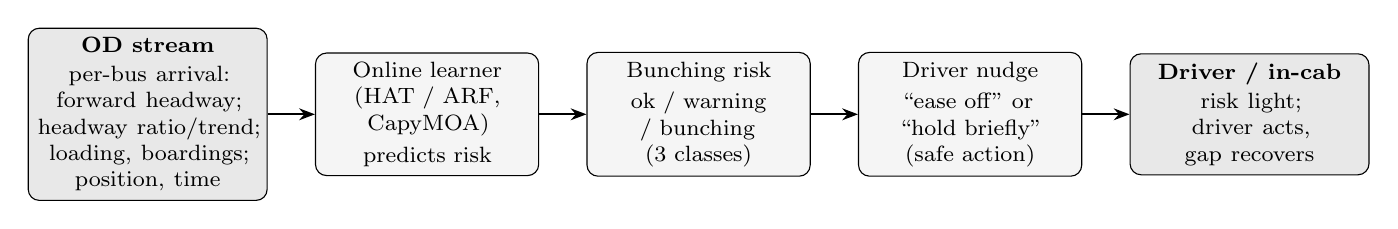
\begin{tikzpicture}[
  node distance=4mm and 6mm,
  box/.style={draw, rounded corners, align=center, font=\footnotesize,
              minimum height=14mm, text width=26mm, fill=gray!8},
  io/.style={draw, rounded corners, align=center, font=\footnotesize\bfseries,
             minimum height=14mm, text width=28mm, fill=gray!18},
  arr/.style={-{Stealth[length=2mm]}, thick}]
\node[io] (data) {OD stream\\[1pt]
  \footnotesize\mdseries per-bus arrival:\\
  forward headway;\\
  headway ratio/trend;\\
  loading, boardings;\\
  position, time};
\node[box, right=of data] (model) {Online learner\\ (HAT / ARF, CapyMOA)\\[2pt]
  \footnotesize\mdseries predicts risk};
\node[box, right=of model] (risk) {Bunching risk\\[2pt]
  \footnotesize\mdseries ok / warning / bunching\\ (3 classes)};
\node[box, right=of risk] (nudge) {Driver nudge\\[2pt]
  \footnotesize\mdseries ``ease off'' or\\ ``hold briefly''\\ (safe action)};
\node[io, right=of nudge] (cab) {Driver / in-cab\\[1pt]
  \footnotesize\mdseries risk light;\\ driver acts,\\ gap recovers};
\draw[arr] (data) -- (model);
\draw[arr] (model) -- (risk);
\draw[arr] (risk) -- (nudge);
\draw[arr] (nudge) -- (cab);
\end{tikzpicture}}
\caption{Runtime flow of the driver-nudge system. The online learner ingests the per-bus features
of each arrival, predicts the next-window bunching risk, and a \texttt{warning} or
\texttt{bunching} class triggers a safe nudge that the driver can act on so the impending bunching
is averted.}
\label{fig:system}
\end{figure}

Table~\ref{tab:worked} makes the chain concrete: as a bus drifts toward the bus ahead, its headway
ratio falls, the model's prediction escalates from \texttt{ok} to \texttt{warning} and then
\texttt{bunching}, and a nudge fires. A warning is only useful, though, if it arrives early enough to
act on. We therefore care about the \emph{nudge lead time}: the gap between the first fired warning
and the first observed bunching on a trip (Figure~\ref{fig:leadtime}). A larger lead time gives the
driver more room to ease off before the buses close up, and it is one of the metrics we report in
Section~\ref{sec:experiments}.

\begin{table}[htbp]
\centering
\caption{Illustrative worked example (not measured) of consecutive arrivals on one trip. As the
headway ratio falls toward the bunching threshold, the model's prediction flips to \texttt{warning}
and then \texttt{bunching}, and a nudge fires. The lead time is the gap from the first fired warning
to the first observed bunching.}
\label{tab:worked}
\footnotesize
\begin{tabular}{ccccccc}
\toprule
Stop & Time & Headway & Headway & True & Model & Nudge \\
(\texttt{pt\_seq}) & (min) & (min) & ratio & label & prediction & fired? \\
\midrule
12 & 0  & 9.8 & 0.98 & ok       & ok       & --- \\
13 & 6  & 7.1 & 0.71 & warning  & warning  & yes (ease off) \\
14 & 11 & 5.4 & 0.54 & warning  & warning  & yes (ease off) \\
15 & 17 & 3.6 & 0.36 & bunching & bunching & yes (ease off) \\
16 & 23 & 2.9 & 0.29 & bunching & bunching & yes (ease off) \\
\bottomrule
\end{tabular}
\end{table}

\begin{figure}[htbp]
\centering
\resizebox{\linewidth}{!}{%
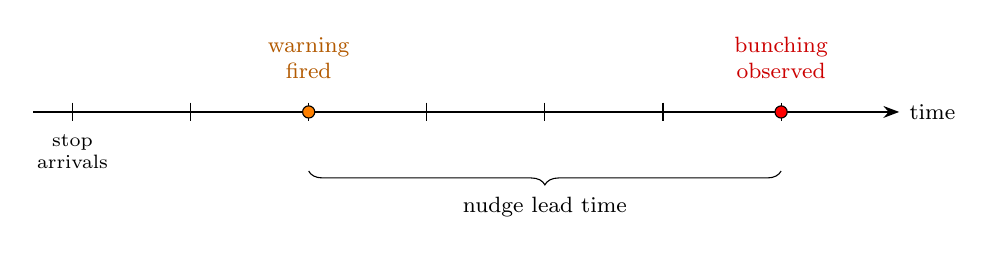
\begin{tikzpicture}[
  font=\footnotesize,
  arr/.style={-{Stealth[length=2mm]}, thick}]
% time axis
\draw[arr] (0,0) -- (11,0) node[right]{time};
% stop arrival ticks
\foreach \x in {0.5,2,3.5,5,6.5,8,9.5}{
  \draw (\x,0.12) -- (\x,-0.12);
}
\node[align=center, font=\scriptsize] at (0.5,-0.5) {stop\\arrivals};
% warning fired marker
\draw[fill=orange] (3.5,0) circle (2.2pt);
\node[orange!70!black, align=center, above=3mm] at (3.5,0) {warning\\fired};
% observed bunching marker
\draw[fill=red] (9.5,0) circle (2.2pt);
\node[red!80!black, align=center, above=3mm] at (9.5,0) {bunching\\observed};
% lead-time brace between them
\draw[decorate, decoration={brace, amplitude=5pt, mirror}] (3.5,-0.75) -- node[below=6pt]{nudge lead time} (9.5,-0.75);
\end{tikzpicture}}
\caption{How nudge lead time is measured (illustrative). Along one trip, it is the elapsed time from
the earliest fired warning to the first observed bunching event. A larger lead time gives the driver
more opportunity to ease off before bunching forms.}
\label{fig:leadtime}
\end{figure}

\subsection{Preprocessing}
\label{sec:preprocessing}

\paragraph{Target format and rationale}
The model does not consume the raw OD rows directly. Preprocessing transforms them into a tidy
\emph{labelled instance stream}: one row per bus arrival at a stop, each carrying a fixed numeric
feature vector and a class label, with all rows sorted by \texttt{stop\_time} into true
chronological order. This format is dictated by the streaming setting. First, prequential
(test-then-train) evaluation requires the data to be a sequence of $(\mathbf{x}_t, y_t)$ events that
can be replayed one at a time in the order they occurred; a row-per-arrival, time-ordered table is
exactly that. Second, chronological order is what prevents leakage: the learner only ever sees the
past before predicting the next arrival, mirroring deployment. Third, the quantity of interest,
the headway, is not a column in OD and must be \emph{derived} (Section~\ref{sec:data}), so a
construction step is unavoidable. Algorithm~\ref{alg:preprocess} gives the procedure,
Figure~\ref{fig:pipeline} the high-level flow, and Table~\ref{tab:feat} the resulting fields.

\begin{algorithm}[H]
\footnotesize
\DontPrintSemicolon
\KwIn{OD event rows; scope (routes, directions, dates); headway window $w$; look-ahead $K$ stops;
      thresholds $\alpha < \beta$ (we use $\alpha{=}0.40$, $\beta{=}0.60$); minimum plausible gap $g$}
\KwOut{\texttt{features.csv}: one labelled instance per bus arrival, sorted by \texttt{stop\_time}}
\BlankLine
Load the OD parquet files for the dates; keep the scoped routes and directions; parse \texttt{stop\_time}\;
\ForEach{trip}{
  \lIf{\texttt{stop\_time} is not non-decreasing along the stop sequence}{discard the trip}
}
\ForEach{trip}{
  compute the segment time to the next stop and the time since the previous stop\;
}
\ForEach{(route, direction, stop), in time order}{
  $h \leftarrow$ arrival time $-$ previous distinct vehicle's arrival time \tcp*[f]{forward headway}\;
  \lIf{$h < g$}{$h \leftarrow$ undefined \tcp*[f]{same-vehicle artefact}}
  $m \leftarrow$ median of the previous $w$ headways at this stop \tcp*[f]{local ``normal''}\;
}
\ForEach{arrival on a trip}{
  $h_{\min} \leftarrow$ minimum forward headway over the next $K$ stops \tcp*[f]{future risk, $>t$}\;
  \uIf{$h_{\min} < \alpha\, m$}{$y \leftarrow$ \emph{bunching}}
  \uElseIf{$h_{\min} < \beta\, m$}{$y \leftarrow$ \emph{warning}}
  \lElse{$y \leftarrow$ \emph{ok}}
}
Engineer the causal features of Table~\ref{tab:feat} (all $\le t$): headway ratio, trend\;
Drop arrivals with no defined headway, normal, or label; replace any non-finite values\;
Sort the surviving rows by \texttt{stop\_time}\;
\caption{Constructing the streaming dataset from SUNT OD.}
\label{alg:preprocess}
\end{algorithm}

\subsection{How the algorithm builds the stream}
\label{sec:build-stream}

In plain terms, Algorithm~\ref{alg:preprocess} walks the OD events once and turns them into a clean,
time-ordered table of labelled examples. It first discards trips whose timestamps are out of order,
since any headway computed from them would be wrong. For every stop it then measures the
\emph{forward headway}, the gap between each bus and the one before it, and a rolling ``normal''
headway for that stop (the median of recent gaps) as a local baseline. Each arrival is then labelled
by looking a few stops ahead: if the bus is about to fall well below its normal spacing it is marked
\emph{bunching}, if it is moderately below it is marked \emph{warning}, and otherwise \emph{ok}.
Crucially the label looks into the future while the features only use the past, so there is no
leakage. Finally the algorithm attaches the causal features, drops arrivals that cannot be labelled
(such as the first bus of the day at a stop), and sorts everything by time.

To make this concrete, we trace the same eleven raw rows of Table~\ref{tab:odsample} through
preprocessing. Table~\ref{tab:feat} lists the columns we engineer from the raw rows into the
modelling table \texttt{data/processed/features.csv} (109{,}029 rows for this scope), and
Table~\ref{tab:featsample} shows those \emph{same} eleven rows after preprocessing, so the reader can
trace raw data straight into the features the model consumes. Boarding and loading counts are
fractional because SUNT \emph{infers} them from fare and vehicle data, so a value like \texttt{2.3}
is expected, not a typo.

As a worked example, follow stop~8 (\texttt{seq}~8) through both tables. In the raw row
(Table~\ref{tab:odsample}) the bus arrives at \texttt{13:30:25} carrying \texttt{load}~2.3.
Preprocessing turns that into the matching row of Table~\ref{tab:featsample}: the arrival time
becomes \texttt{min\_day}~$=810$ (since $13\times60+30=810$); the gap to the previous bus at this
same stop is \texttt{headway}~$=15.8$~min, while the local ``normal'' there is
\texttt{normal}~$=39.4$~min, so \texttt{ratio}~$=15.8/39.4\approx0.40$, meaning the bus is at about
$40\%$ of its usual spacing, i.e.\ closing on the bus ahead; the time since the previous stop is
\texttt{since\_prev}~$=1.0$~min (from \texttt{13:29:25} to \texttt{13:30:25}); the onboard load
carries over as \texttt{load}~$=2.26$ (the same 2.3, at full precision); the date is a Friday so
\texttt{dow}~$=4$, and 13:30 is outside the commute peaks so \texttt{peak}~$=0$. Finally the
\texttt{label} is~$1$ (warning): looking a few stops ahead, the headway is about to fall further
toward the bunching threshold. In short, one raw OD arrival becomes one row of model-ready numbers.

\begin{table}[H]
\centering
\small
\caption{Engineered columns in \texttt{features.csv}. ``Causal'' columns use only the past
($\le$ now); the \texttt{label} looks into the future and is the prediction target, never an input.}
\label{tab:feat}
\begin{tabular}{P{3.2cm}P{1.5cm}P{8.2cm}}
\toprule
Column & Role & Meaning (plain English) \\
\midrule
\texttt{headway\_min}          & feature & Minutes since the \emph{previous} bus passed this same stop, the gap to the bus ahead. \\
\texttt{local\_median\_headway}& reference & The ``normal'' gap here: the median of the last 8 gaps at this stop. \\
\texttt{headway\_ratio}        & feature & \texttt{headway\_min} $\div$ normal. Below~1 = closer than usual (bunching). \\
\texttt{headway\_trend}        & feature & Change in the gap versus the previous bus at this stop (closing or opening). \\
\texttt{since\_prev\_stop\_min}& feature & Minutes this bus took to get here from its previous stop (running-time proxy). \\
\texttt{pt\_sequence}          & feature & Position along the route. \\
\texttt{is\_peak}              & feature & 1 during the commute peaks (06--08h, 17--19h), else 0. \\
\texttt{label}                 & target  & \{0 ok, 1 warning, 2 bunching\}: is the gap about to collapse below 60\%/40\% of normal within the next 3 stops? \\
\bottomrule
\end{tabular}
\end{table}

\begin{table}[H]
\centering
\setlength{\tabcolsep}{4pt}
\scriptsize
\caption{The engineered \texttt{features.csv} rows computed from the \emph{same} eleven raw OD rows
of Table~\ref{tab:odsample} (trip 20407\_1007\_2). Read the two tables together:
Table~\ref{tab:odsample} is the raw input, this is what the model sees after preprocessing
(Table~\ref{tab:feat} defines each column). Abbreviations: \texttt{seq}~=~pt\_sequence,
\texttt{headway}~=~headway\_min, \texttt{normal}~=~local\_median\_headway,
\texttt{ratio}~=~headway\_ratio, \texttt{trend}~=~headway\_trend,
\texttt{since\_prev}~=~since\_prev\_stop\_min,
\texttt{peak}~=~is\_peak. Note how the raw \texttt{stop\_time}
of Table~\ref{tab:odsample} turns into the per-stop gaps and into
\texttt{since\_prev}; and a bunched
\texttt{ratio} ($\approx$0.4) yields warning (1) or bunching (2) labels. The shaded row
(\texttt{seq}~8) is the one traced in the worked example.}
\label{tab:featsample}
\begin{tabular}{rrrrrrrrr}
\toprule
seq & headway & normal & ratio & trend & since\_prev & min\_day & peak & label \\
\midrule
1  & 18.07 & 37.00 & 0.49 & -11.88 & 0.00 & 4 & 0 & 1 \\
2  & 18.13 & 37.14 & 0.49 & -12.08 & 0.33 & 4 & 0 & 1 \\
3  & 16.87 & 38.92 & 0.43 & -17.93 & 3.33 & 4 & 0 & 1 \\
4  & 16.75 & 39.02 & 0.43 & -19.32 & 1.17 & 4 & 0 & 1 \\
5  & 16.25 & 39.36 & 0.41 & -21.30 & 1.00 & 4 & 0 & 1 \\
6  & 16.22 & 40.14 & 0.40 & -22.53 & 1.18 & 4 & 0 & 2 \\
7  & 15.75 & 40.48 & 0.39 & -23.80 & 0.35 & 4 & 0 & 2 \\
\rowcolor{gray!15} 8  & 15.82 & 39.43 & 0.40 & -22.55 & 1.00 & 4 & 0 & 1 \\
9  & 16.35 & 38.34 & 0.43 & -21.42 & 1.87 & 4 & 0 & 1 \\
10 & 16.33 & 38.38 & 0.43 & -21.47 & 0.35 & 4 & 0 & 1 \\
11 & 16.35 & 34.40 & 0.48 & -10.13 & 0.80 & 4 & 0 & 1 \\
\bottomrule
\end{tabular}
\end{table}

The output is \texttt{features.csv}: one row per bus arrival, in the exact order the arrivals
happened. This file \emph{is} the stream that the learners consume in Section~\ref{sec:experiments}.
They read it one row at a time and, for each arrival, first predict the bunching class from the
features and then learn from the true label, mirroring how the system would run live (prequential,
test-then-train). Because the table is already ordered and labelled, no further reshaping is needed:
the preprocessing is what turns raw operational data into something a streaming model can learn from
online.

\begin{figure}[htbp]
\centering
\resizebox{\linewidth}{!}{%
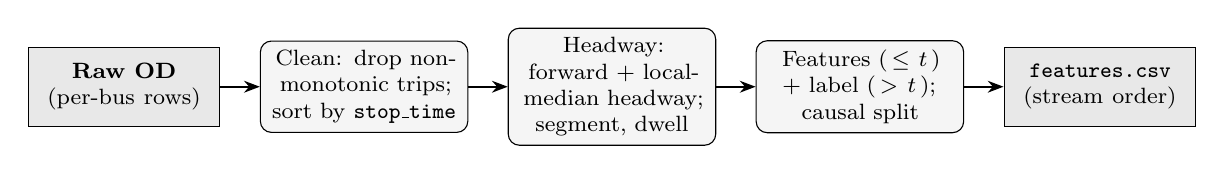
\begin{tikzpicture}[
  node distance=4mm and 5mm,
  box/.style={draw, rounded corners, align=center, font=\footnotesize,
              minimum height=10mm, text width=24mm, fill=gray!8},
  io/.style={draw, align=center, font=\footnotesize\bfseries,
             minimum height=10mm, text width=22mm, fill=gray!18},
  arr/.style={-{Stealth[length=2mm]}, thick}]
\node[io] (od) {Raw OD\\ \footnotesize\mdseries (per-bus rows)};
\node[box, right=of od] (clean) {Clean: drop non-monotonic trips; sort by \texttt{stop\_time}};
\node[box, right=of clean] (head) {Headway: forward + local-median headway; segment, dwell};
\node[box, right=of head] (feat) {Features (\,$\le t$\,) $+$ label (\,$>t$\,); causal split};
\node[io, right=of feat] (csv) {\texttt{features.csv}\\ \footnotesize\mdseries (stream order)};
\draw[arr] (od) -- (clean);
\draw[arr] (clean) -- (head);
\draw[arr] (head) -- (feat);
\draw[arr] (feat) -- (csv);
\end{tikzpicture}}
\caption{Preprocessing pipeline from the raw SUNT OD data to the modelling table. Each stage is a
function in the submitted code; the output is replayed chronologically for prequential evaluation.}
\label{fig:pipeline}
\end{figure}

\subsection{Counterfactual simulation design}
\label{sec:simdesign}

Predicting bunching is only useful if acting on the prediction would change the outcome, yet the
true effect of drivers easing off cannot be observed from historical data: the public SUNT release
contains no period in which the copilot was deployed. We therefore design a \emph{counterfactual
simulation} that re-runs the actual headway geometry under a small, bounded behavioural change,
rather than asserting an effect. This subsection specifies the procedure; its results are reported
in Section~\ref{sec:after} and interpreted in Section~\ref{sec:discussion}.

The simulation replays the recorded arrival stream in time order. Whenever the deployed ARF fires a
nudge on a bus that is genuinely \emph{closing} on the one ahead (headway ratio below the warning
threshold), the driver eases off: we add a small bounded delay --- a few seconds per stop, capped at
$1.5$~min per trip --- to that bus's subsequent arrivals, then recompute the downstream forward
headways and re-measure bunching, headway $\mathrm{CV}$, and excess wait (Eq.~\ref{eq:excess}). The
ease-off magnitude is the decentralised analogue of the small adaptive holds of \citet{Daganzo2009}
and the advisory counterpart of the cooperative speed control of \citet{DaganzoPilachowski2011}, in
which a leading bus slows for the one behind and is never asked to speed up. It is also consistent
with \citet{Enayatollahi2019}, who show that shaving a little dwell per stop materially reduces
bunching. The nudge never asks a driver to speed up, and the local ``normal'' headway is held at its
baseline value so the comparison is against a fixed reference.
Algorithm~\ref{alg:counterfactual} states the procedure.

\begin{algorithm}[H]
\footnotesize
\DontPrintSemicolon
\KwIn{recorded arrivals with model predictions; ease-off $\delta$ (s); per-trip cap $C$;
      closing threshold $\tau$; mode $\in$ \{all-fired, true-positive-only\}}
\KwOut{counterfactual bunching count, headway CV, and excess wait vs.\ baseline}
\BlankLine
$\textit{delay}[\textit{trip}] \leftarrow 0$ for all trips\;
\ForEach{arrival $a$ in trip order}{
  $t'[a] \leftarrow \texttt{stop\_time}[a] + \textit{delay}[\textit{trip}(a)]$ \tcp*[f]{shift by accumulated ease-off}\;
  $\textit{fired} \leftarrow (\text{prediction}[a] \ge \text{warning})$\;
  \lIf{mode $=$ true-positive-only}{$\textit{fired} \leftarrow \textit{fired} \wedge (\text{label}[a] \ge \text{warning})$}
  $\textit{closing} \leftarrow (\text{headway ratio}[a] < \tau)$\;
  \If{$\textit{fired} \wedge \textit{closing} \wedge \textit{delay}[\textit{trip}(a)] < C$}{
    $\textit{delay}[\textit{trip}(a)] \leftarrow \min(\textit{delay}[\textit{trip}(a)] + \delta,\; C)$\;
  }
}
recompute forward headways on the shifted times $t'$; recompute bunching, CV, excess wait\;
\caption{Counterfactual ease-off replay (simulation).}
\label{alg:counterfactual}
\end{algorithm}

To keep the estimate honest we build in two robustness checks, reported in Section~\ref{sec:after}:
an \emph{ablation} that gates the ease-off to only the model's \emph{correct} (true-positive)
predictions, isolating the contribution of real-time prediction from hindsight; and a
\emph{sensitivity sweep} of the per-stop ease-off magnitude, testing whether the result depends on
one chosen value. Two effects are deliberately outside the simulation's reach: real driver compliance
and the true human response are not in historical data, so the result is an estimate under stated
assumptions rather than a measured field outcome; and bus occupancy and stop boardings have no
measurable link to spacing in SUNT ($r\approx0.09$ and $r\approx0.00$), so we do not simulate a
crowding benefit.

%% ======================================================================
\section{Experiments}
\label{sec:experiments}

\paragraph{Setup}
We reconstruct per-bus trajectories from OD, compute forward headways per
route$\times$direction$\times$stop, build the causal features and the forward-looking label,
and replay all events chronologically by \texttt{stop\_time}. The reported run scopes to the
eight busiest routes on 1~March 2024 --- 1007, 1386, 1346, 1649, 12503, 1320, 1637 and 1413 ---
over 1--3 March 2024 (109{,}029 instances; class balance: ok~70\%, warning~10\%, bunching~20\%).
Trips with non-monotonic \texttt{stop\_time} ($\approx$23\% at this scope) are dropped.
Before modelling we establish, purely descriptively, that bunching is a real and costly problem
on these routes (Section~\ref{sec:before}).

\paragraph{Evaluation}
We use \emph{prequential} (test-then-train) evaluation in strict chronological order: the model
predicts for the bus about to arrive, the bus arrives, the model learns from the realised
outcome, then predicts the next. Random train/test splits would leak the future and are avoided.
Because bunching is the rare positive class, we report imbalance-aware metrics --- precision,
recall, and F1 on the bunching class, plus balanced accuracy and Cohen's $\kappa$ --- following
established practice for evaluating imbalanced data streams \citep{Aguiar2024}, where accuracy
alone is misleading under a drifting class ratio. We also report the
\emph{nudge lead time}: the minutes between a fired warning and the observed bunching
(introduced in Section~\ref{sec:system}, Figure~\ref{fig:leadtime}).

\paragraph{Baselines and bake-off}
The streaming models are compared against deliberately simple alternatives: a static
headway-threshold rule (``is the gap small right now?''), previous-headway persistence, and a
majority-class floor. We then run a bake-off of CapyMOA classifiers on the same stream:
Naive Bayes, $k$-Nearest Neighbours, Hoeffding Tree, Extremely Fast Decision Tree (EFDT),
Hoeffding Adaptive Tree (HAT), and Adaptive Random Forest (ARF).

\paragraph{Hyperparameters}
ARF uses an ensemble size of 25 and Poisson $\lambda = 6$; trees use a grace period of 200;
ADWIN uses $\delta = 0.002$. A fixed random seed is reported for reproducibility.

\subsection{Bake-off results}
\label{sec:bakeoff}

We first report which learner predicts bunching best, and early enough to act on, before turning to
the service-quality measurements in Section~\ref{sec:results}. Table~\ref{tab:bakeoff} ranks the
candidates by bunching-class F1. ARF attains the best F1 (0.916), balanced accuracy (0.915), and
$\kappa$ (0.892), ahead of the single adaptive tree (HAT) and the static threshold. The non-learning
Naive Bayes and majority-class floor collapse to the majority class and score zero on the bunching
class. There is a clear accuracy-versus-throughput trade-off: HAT processes roughly an order of
magnitude more instances per second than ARF for about one F1 point less, which matters for an in-cab
deployment.

\begin{table}[t]
\centering
\caption{Prequential model bake-off (bunching class), 109{,}029 instances. Ranked by F1.
The static threshold is a non-learning reference.}
\label{tab:bakeoff}
\begin{tabular}{lccccc}
\toprule
Model & F1 & Recall & Bal.\ acc. & $\kappa$ & inst./s \\
\midrule
\textbf{ARF}                 & \textbf{0.916} & 0.915 & 0.915 & 0.892 & 6{,}162 \\
static threshold (ref.)      & 0.909 & 0.890 & 0.904 & 0.883 & --- \\
HAT                          & 0.907 & 0.901 & 0.899 & 0.879 & 57{,}658 \\
Hoeffding Tree               & 0.886 & 0.848 & 0.791 & 0.792 & 71{,}790 \\
EFDT                         & 0.877 & 0.836 & 0.789 & 0.785 & 63{,}120 \\
KNN                          & 0.761 & 0.721 & 0.728 & 0.676 & 11{,}575 \\
Naive Bayes                  & 0.000 & 0.000 & 0.333 & 0.000 & 97{,}835 \\
Majority class               & 0.000 & 0.000 & 0.334 & 0.002 & 86{,}598 \\
\bottomrule
\end{tabular}
\end{table}

Crucially, the streaming models warn \emph{ahead of time}. ARF's nudges fire a median of
$\approx$28~minutes before the observed bunching (Fig.~\ref{fig:lead}), whereas the static
threshold and persistence baselines have no meaningful lead --- they detect bunching as it
happens rather than predicting it, so they cannot support a useful driver nudge. Figure~\ref{fig:roll}
shows prequential accuracy over the stream with ADWIN drift markers, confirming the adaptive learners
recover after distribution shifts.

\begin{figure}[t]
\centering
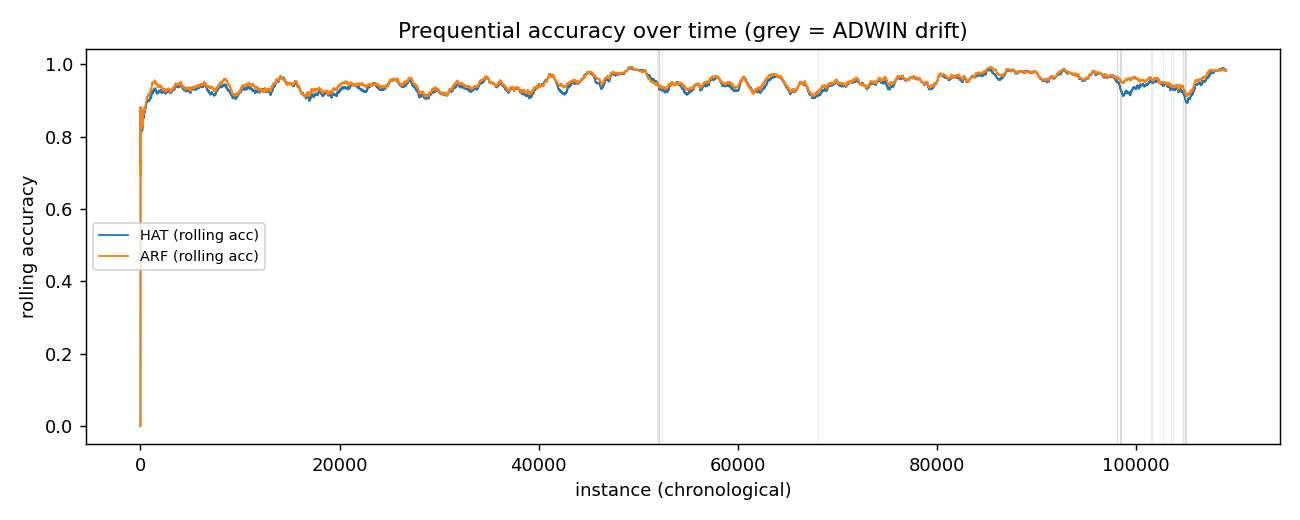
\includegraphics[width=\linewidth]{figures/rolling_accuracy.png}
\caption{Prequential accuracy over the chronological stream for HAT and ARF; grey lines mark
ADWIN-detected drift points.}
\label{fig:roll}
\end{figure}

\begin{figure}[t]
\centering
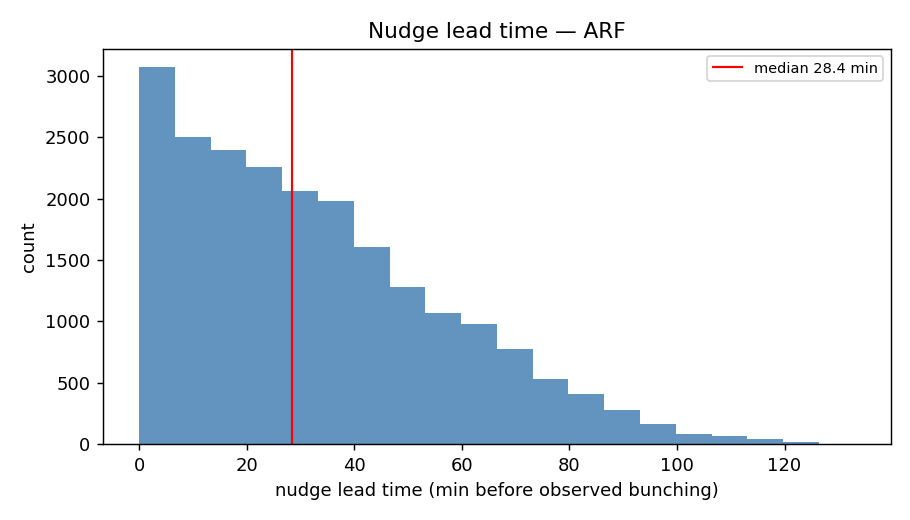
\includegraphics[width=0.75\linewidth]{figures/lead_time_hist.png}
\caption{Nudge lead time for ARF: minutes between a fired warning and the observed bunching.}
\label{fig:lead}
\end{figure}

%% ======================================================================
\section{Results}
\label{sec:results}

Having selected a model that predicts bunching with actionable lead time
(Section~\ref{sec:bakeoff}), we now measure the service-quality effect. We present this as a
\emph{before/after} comparison: Section~\ref{sec:before} measures how bunched the recorded service
already is (the ``before''), and Section~\ref{sec:after} re-runs each of those measurements on the
counterfactual ``after'' (Section~\ref{sec:simdesign}), stating for each whether it improved.
Section~\ref{sec:after} mirrors Section~\ref{sec:before} measurement-for-measurement, and
Table~\ref{tab:mirror} maps the pairs and their verdicts at a glance.

\subsection{Before: bunching in the recorded data}
\label{sec:before}

We first establish, \emph{descriptively and without machine learning}, that bunching is a real and
costly problem on these routes, measuring it directly from the reconstructed forward headways. To
avoid mistaking the natural daily demand cycle (short peak gaps, long late-evening gaps) for
bunching, every statistic is computed \emph{within} hourly windows --- per route, direction, stop and
hour-of-day --- so we compare like-with-like demand. We report six measurements; the same six are
re-run after the nudge in Section~\ref{sec:after}.

\subsubsection{Headway irregularity (CV)}
\label{sec:b-cv}
The standard measure of spacing irregularity is the headway coefficient of variation
$\mathrm{CV} = \mathrm{std}(h)/\mathrm{mean}(h)$: $\mathrm{CV}=0$ is perfectly even service and
bunching inflates it. Across the eight routes the median within-window $\mathrm{CV}$ is $0.73$
(mean $0.80$); the irregularity is worse in the peak, where most passengers travel, rising from
$0.79$ off-peak to $0.86$ in the peak (Fig.~\ref{fig:cv}).

\subsubsection{How close the buses run (headway ratio)}
\label{sec:b-ratio}
For every arrival we compute the headway ratio (realised gap divided by the local-normal gap). By the
same thresholds the model uses, $19.4\%$ of arrivals are already bunched (ratio $<0.40$) and a further
$9.8\%$ are in warning (ratio $<0.60$); the full distribution is Fig.~\ref{fig:ratiohist}.

\subsubsection{Avoidable passenger waiting}
\label{sec:b-wait}
We convert this irregularity into a concrete cost --- minutes of avoidable waiting. For a stop served
at headways $h_i$, the mean wait of a passenger arriving at random (Poisson) is the renewal-theory
result
\begin{equation}
\mathbb{E}[W] \;=\; \frac{\mathbb{E}[h^2]}{2\,\mathbb{E}[h]}
            \;=\; \frac{\bar h}{2}\bigl(1 + \mathrm{CV}^2\bigr),
\label{eq:wait}
\end{equation}
whose first term $\bar h/2$ is the wait under perfectly even service. The remainder is therefore the
\emph{avoidable} wait caused purely by irregularity,
\begin{equation}
W_{\mathrm{excess}} \;=\; \frac{\bar h}{2}\,\mathrm{CV}^2 .
\label{eq:excess}
\end{equation}
Applying Eq.~\eqref{eq:excess} per window and weighting by boardings, irregular spacing on these eight
routes imposes on the order of $5.6\times10^{5}$ avoidable passenger-waiting-minutes per day
($\approx 9{,}400$ passenger-hours daily), with a mean of $\approx 17$ avoidable minutes per waiting
passenger (Fig.~\ref{fig:excess}).

\subsubsection{Severity over the day}
\label{sec:b-sev}
Following \citet{Enayatollahi2019}, we track a per-arrival severity $\max(0,\,1-\text{headway ratio})$,
which is $0$ on schedule and rises toward $1$ as a bus closes up on the one ahead. Averaged by hour it
peaks in the morning and evening commute (Fig.~\ref{fig:severity}), so bunching concentrates exactly
when buses are fullest.

\subsubsection{Seeing bunching directly (string diagram)}
\label{sec:b-string}
The per-bus string diagram (Fig.~\ref{fig:string}) shows the same phenomenon in the raw trajectories:
time runs along the horizontal axis and a bus's position along the route up the vertical axis, so each
line follows one bus, and where lines converge or cross those buses are bunching. This structure is
visible only because OD records each bus individually with exact arrival times, and would vanish under
5-/30-minute aggregation (Section~\ref{sec:data}).

\subsubsection{Travel-time context (congestion, not a nudge target)}
\label{sec:b-travel}
For completeness we also record terminal-to-terminal ride time
(\texttt{end\_trip} $-$ \texttt{start\_trip}), which is longer at peak on most routes
(Table~\ref{tab:travel}): route 1007 is $+18.4\%$, the network median $+2.7\%$. This is ordinary road
congestion. We include it as context only: the nudge evens \emph{spacing}, not driving speed, so this
is explicitly \emph{not} a quantity we expect it to improve --- a point we make good on in
Section~\ref{sec:a-travel}.

\begin{table}[htbp]
\centering
\small
\caption{Travel-time context (``before''): median terminal-to-terminal trip time, peak versus
off-peak. Real congestion, but not a target of the nudge (cf.\ Section~\ref{sec:a-travel}).}
\label{tab:travel}
\begin{tabular}{lrrr}
\toprule
Route & Peak (min) & Off-peak (min) & $\Delta$ \\
\midrule
1007  & 99.5 & 84.1 & $+18.4\%$ \\
1346  & 49.5 & 45.0 & $+9.9\%$  \\
1413  & 88.1 & 82.8 & $+6.4\%$  \\
1320  & 66.3 & 65.0 & $+2.0\%$  \\
12503 & 95.0 & 93.4 & $+1.7\%$  \\
1386  & 92.6 & 91.1 & $+1.6\%$  \\
1649  & 83.3 & 84.1 & $-0.9\%$  \\
1637  & 78.1 & 79.1 & $-1.3\%$  \\
\bottomrule
\end{tabular}
\end{table}

\begin{figure}[htbp]
\centering
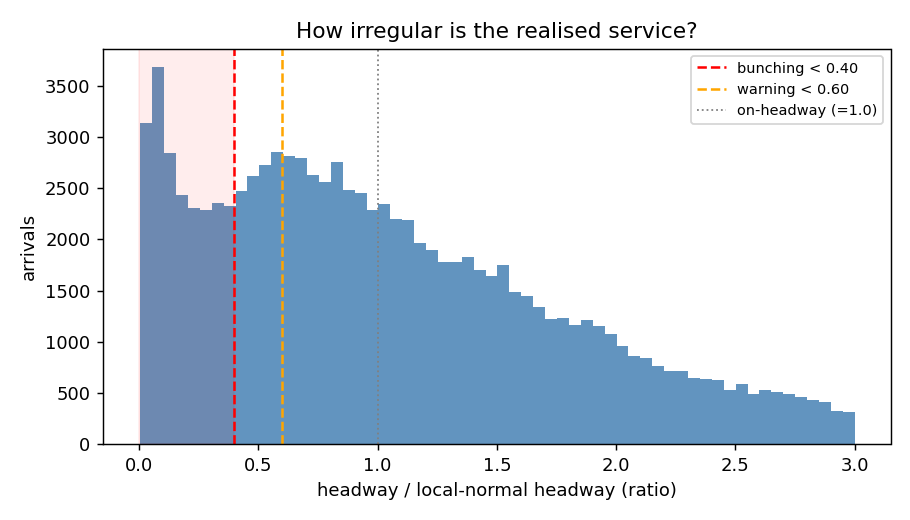
\includegraphics[width=0.8\linewidth]{figures/headway_ratio_hist.png}
\caption{Distribution of the realised headway as a fraction of the local-normal headway.
Mass left of the dashed lines is service that is in warning ($<0.60$) or bunched ($<0.40$).}
\label{fig:ratiohist}
\end{figure}

\begin{figure}[htbp]
\centering
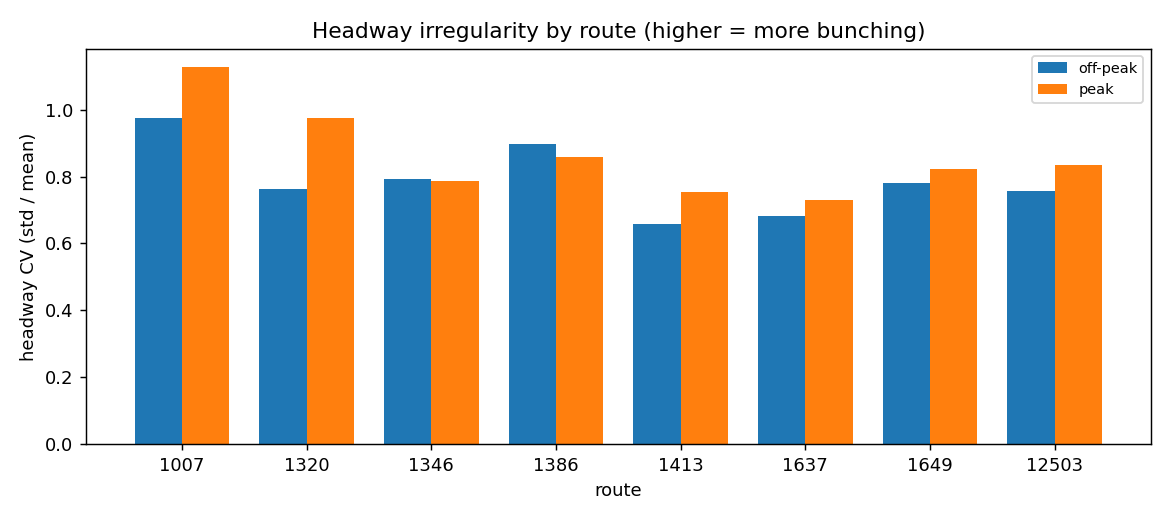
\includegraphics[width=0.9\linewidth]{figures/headway_cv_by_route.png}
\caption{Within-window headway coefficient of variation per route, peak versus off-peak. Higher
is more irregular; the peak is consistently worse.}
\label{fig:cv}
\end{figure}

\begin{figure}[htbp]
\centering
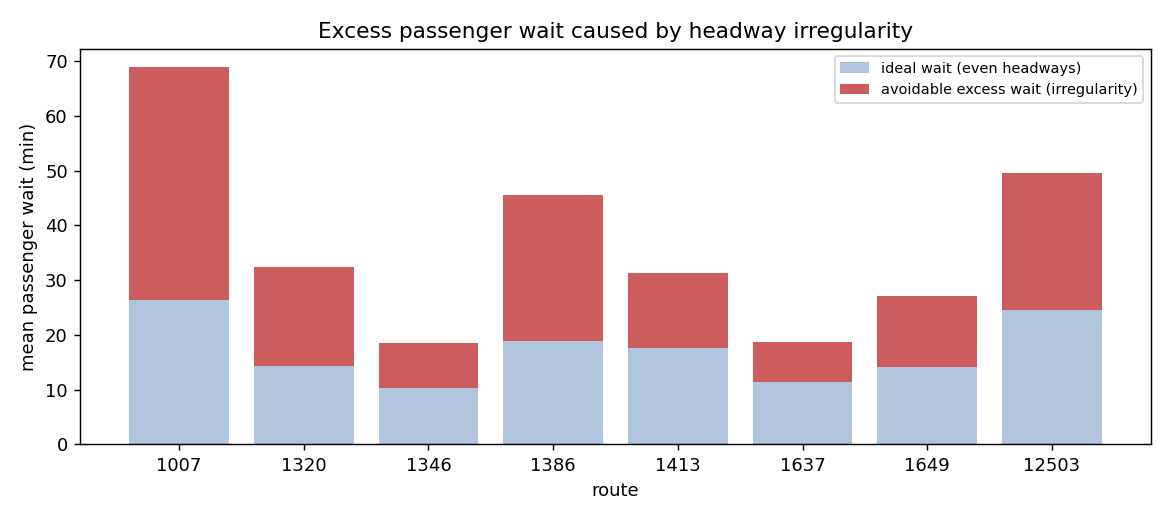
\includegraphics[width=0.9\linewidth]{figures/excess_wait_by_route.png}
\caption{Mean passenger wait per route decomposed into the even-headway ideal ($\bar h/2$) and
the \emph{avoidable} excess caused by irregularity (Eq.~\ref{eq:excess}).}
\label{fig:excess}
\end{figure}

\begin{figure}[htbp]
\centering
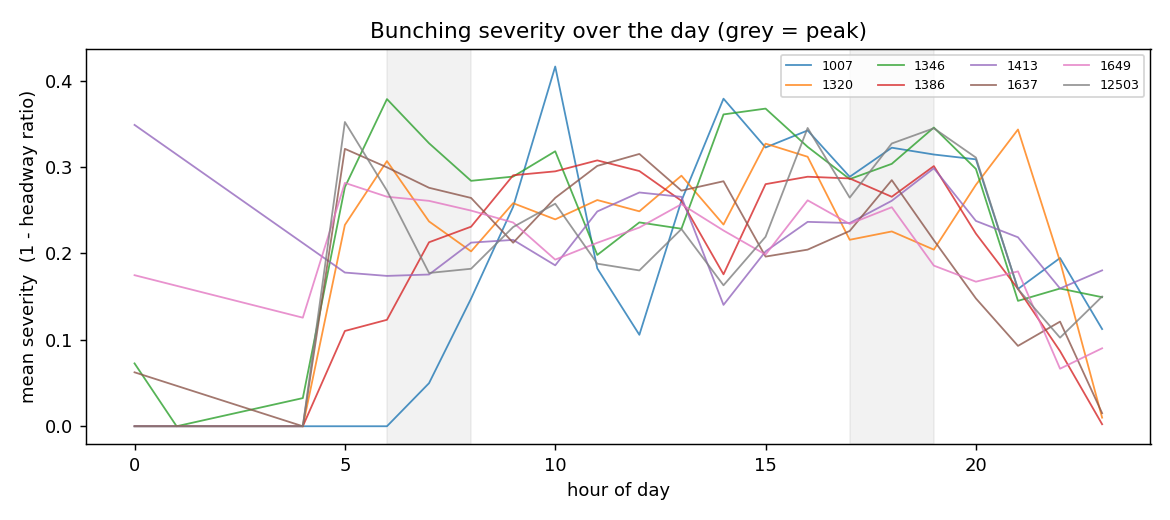
\includegraphics[width=0.9\linewidth]{figures/severity_timeseries.png}
\caption{Mean bunching severity ($\max(0,1-\text{headway ratio})$) by hour of day, per route;
shaded bands are the morning and evening peaks.}
\label{fig:severity}
\end{figure}

\begin{figure}[t]
\centering
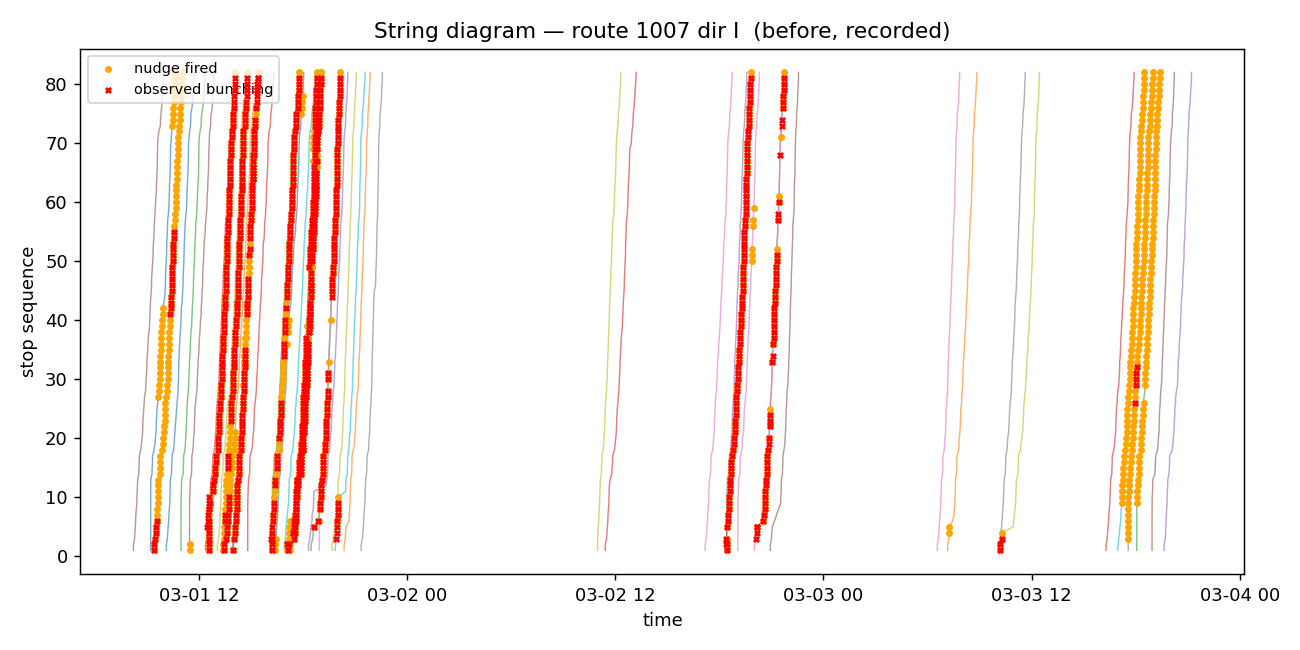
\includegraphics[width=\linewidth]{figures/string_diagram.png}
\caption{Per-bus trajectories (``string diagram'') for one route reconstructed from raw OD.
Each line is one bus over time; converging or crossing lines are bunching events. Orange/red
markers show fired nudges and observed bunching. The signal exists because OD keeps individual
vehicles and exact timestamps; aggregation into per-interval counts destroys it.}
\label{fig:string}
\end{figure}

\subsection{After: the same measurements, after the nudge}
\label{sec:after}

We now re-run the six ``before'' measurements of Section~\ref{sec:before} on the simulated ``after''
arrival times (the counterfactual of Section~\ref{sec:simdesign}). The subsections below mirror
Section~\ref{sec:before} one-to-one, each stating whether that measurement improved;
Table~\ref{tab:mirror} summarises the verdicts and Table~\ref{tab:panel} gives the full numeric
panel. Under the default ease-off ($8$~s per nudged stop), the simulation rests on $\approx$$11{,}000$
small ease-offs, and two robustness checks support it: an \emph{ablation} that gates the ease-off to
only the model's \emph{correct} (true-positive) nudges yields virtually the same reduction
($-12.7\%$ bunching / $-9.8\%$ wait), so the benefit is driven by the model's predictions rather than
hindsight; and a \emph{sensitivity sweep} of the ease-off magnitude from $4$ to $16$~s leaves the
reduction in a narrow $12$--$13\%$ band (Fig.~\ref{fig:cfsens}).

\begin{table}[htbp]
\centering
\small
\caption{Each ``before'' measurement (Section~\ref{sec:before}) and its matching ``after''
subsection (Section~\ref{sec:after}), with the verdict.}
\label{tab:mirror}
\begin{tabular}{lll}
\toprule
Before & After & Verdict \\
\midrule
Headway irregularity (CV)        & §\ref{sec:a-cv}     & improves ($-3.5\%$) \\
How close the buses run (ratio)  & §\ref{sec:a-ratio}  & improves ($-11.2\%$ / $-12.6\%$) \\
Avoidable passenger waiting      & §\ref{sec:a-wait}   & improves ($-9.8\%$) \\
Severity over the day            & §\ref{sec:a-sev}    & improves \\
Seeing bunching (string diagram) & §\ref{sec:a-string} & improves \\
Travel-time context              & §\ref{sec:a-travel} & not a target (unchanged) \\
\bottomrule
\end{tabular}
\end{table}

\begin{table}[htbp]
\centering
\small
\caption{Before (actual March 2024) versus after (counterfactual nudge), from $\approx$$11{,}000$
ease-offs. ``Improvement'' is the reduction from before to after. The lower block lists indicators
that the nudge is not designed to move (it evens spacing, it is not a speed-up).}
\label{tab:panel}
\begin{tabular}{lrrr}
\toprule
Indicator & Before & After & Improvement \\
\midrule
\multicolumn{4}{l}{\textit{Improves with the nudge}}\\
Bunching events (count)            & 21{,}123 & 18{,}463 & $-12.6\%$ \\
Bunching rate (\% of arrivals)     & 19.4\%   & 17.2\%   & $-11.2\%$ \\
Avoidable wait (passenger-min)     & 201{,}978& 182{,}196& $-9.8\%$  \\
Headway irregularity (mean CV)     & 0.796    & 0.768    & $-3.5\%$  \\
\midrule
\multicolumn{4}{l}{\textit{Checked, but no improvement (the nudge is not a speed-up)}}\\
Mean headway deviation (min)       & 25.4     & 25.1     & $-1.0\%$  \\
Median wait (min)                  & 10.7     & 10.7     & $\approx 0$ \\
Wait spread (std, min)             & 33.9     & 34.1     & $+0.4\%$  \\
\bottomrule
\end{tabular}
\end{table}

\subsubsection{Headway irregularity (CV) --- improves}
\label{sec:a-cv}
\emph{Mirrors Section~\ref{sec:b-cv}.} The mean headway $\mathrm{CV}$ falls $0.796 \to 0.768$
($-3.5\%$; middle panel of Fig.~\ref{fig:cf}). The improvement is modest because the nudge removes the
short-gap bunching it targets but leaves the long late-evening gaps, which dominate the raw spread,
untouched.

\subsubsection{How close the buses run --- improves}
\label{sec:a-ratio}
\emph{Mirrors Section~\ref{sec:b-ratio}.} The share of arrivals that are bunched falls from $19.4\%$
to $17.2\%$ ($-11.2\%$), and the raw count of bunching events from $21{,}123$ to $18{,}463$
($-12.6\%$; left panel of Fig.~\ref{fig:cf}). This is the headline result: about one bunching event in
eight does not form, because a closing bus eased off and let the gap reopen.

\subsubsection{Avoidable passenger waiting --- improves}
\label{sec:a-wait}
\emph{Mirrors Section~\ref{sec:b-wait}.} Avoidable wait drops from $201{,}978$ to $182{,}196$
passenger-minutes ($-9.8\%$; right panel of Fig.~\ref{fig:cf}). The \emph{median} wait itself barely
moves ($\approx$$10.7$~min before and after), because easing a closing bus off slightly delays it; the
benefit is concentrated in the avoidable, variance-driven portion of the wait rather than the average
(Section~\ref{sec:discussion} develops this point).

\subsubsection{Severity over the day --- improves}
\label{sec:a-sev}
\emph{Mirrors Section~\ref{sec:b-sev}.} The ``after'' severity curve sits at or below the ``before''
curve at every hour (Fig.~\ref{fig:sevafter}), with the largest gap during the commute peaks. Severity
falls automatically when there are fewer closed-up arrivals, so this is the same effect as the bunching
reduction, now seen across the day.

\subsubsection{Seeing bunching directly (string diagram) --- improves}
\label{sec:a-string}
\emph{Mirrors Section~\ref{sec:b-string}.} On the counterfactual arrival times fewer bus-lines converge
into platoons than in the recorded diagram (Fig.~\ref{fig:stringafter} versus Fig.~\ref{fig:string}).
The change is visible but subtle, as expected for a roughly one-in-eight reduction rather than a total
fix.

\subsubsection{Travel-time context --- not a target}
\label{sec:a-travel}
\emph{Mirrors Section~\ref{sec:b-travel}.} Unchanged by design. The nudge never speeds a bus up, so
terminal-to-terminal ride time is not affected and the peak-versus-off-peak congestion of
Table~\ref{tab:travel} is untouched. We report it only so the before/after pairing is complete, not as
a claimed improvement.

\begin{figure}[htbp]
\centering
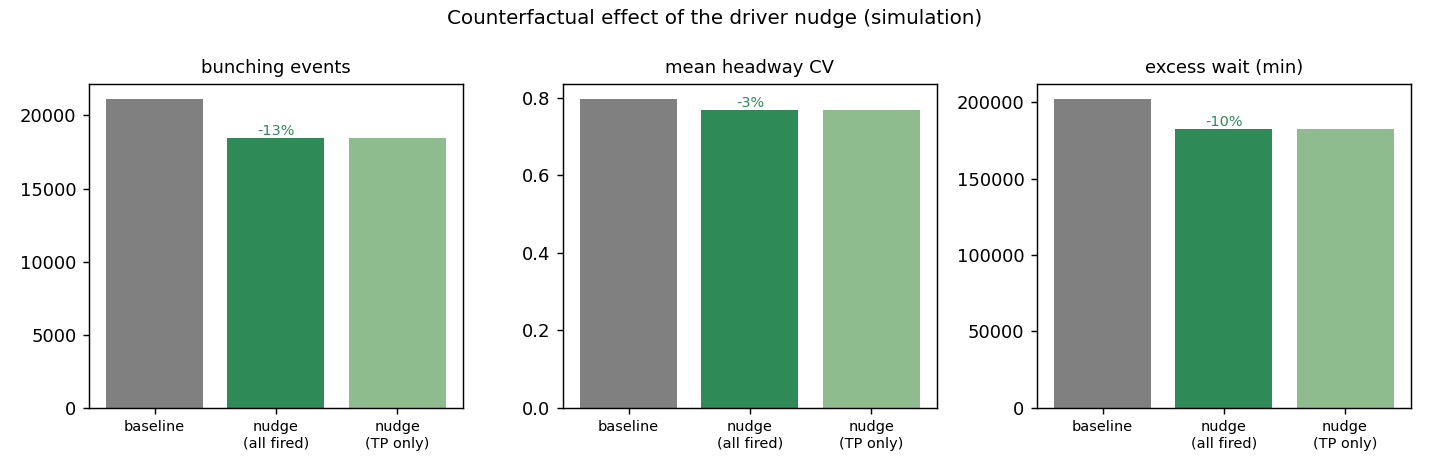
\includegraphics[width=\linewidth]{figures/counterfactual_comparison.png}
\caption{Counterfactual effect of the nudge (simulation): bunching events, headway CV, and
avoidable wait, for the baseline versus the nudge applied on all fired warnings and on
true-positive warnings only.}
\label{fig:cf}
\end{figure}

\begin{figure}[htbp]
\centering
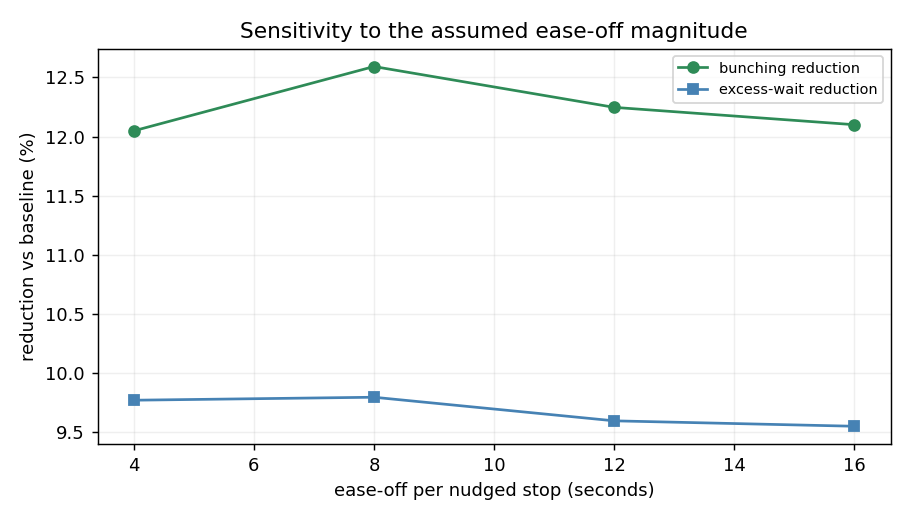
\includegraphics[width=0.8\linewidth]{figures/counterfactual_sensitivity.png}
\caption{Sensitivity of the simulated reduction in bunching and in excess wait to the assumed
per-stop ease-off magnitude. The effect is stable across $4$--$16$~s.}
\label{fig:cfsens}
\end{figure}

\begin{figure}[htbp]
\centering
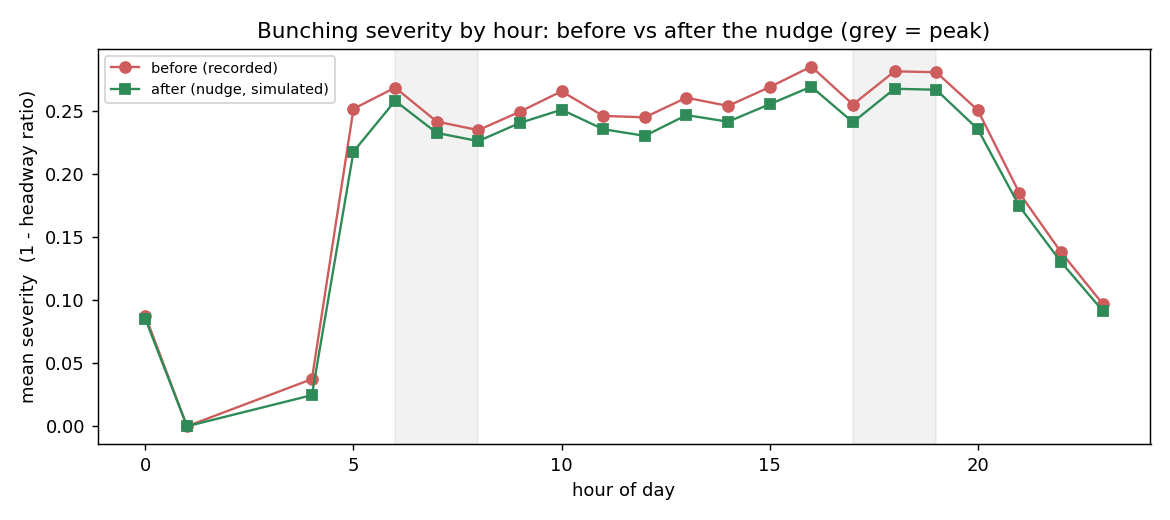
\includegraphics[width=0.9\linewidth]{figures/severity_timeseries_after.png}
\caption{Bunching severity by hour, before (recorded) versus after (simulated nudge). The
``after'' curve sits at or below the ``before'' curve all day; shaded bands are the morning and
evening commute peaks.}
\label{fig:sevafter}
\end{figure}

\begin{figure}[htbp]
\centering
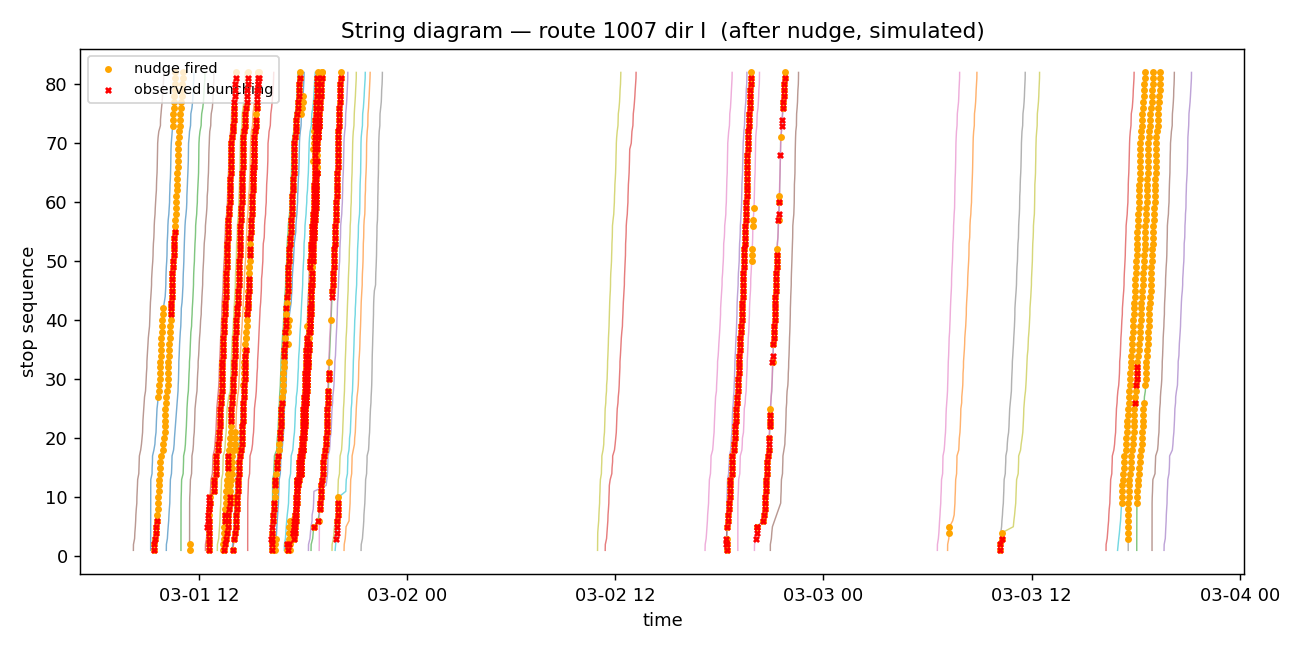
\includegraphics[width=0.9\linewidth]{figures/string_diagram_after.png}
\caption{Per-bus trajectories on the simulated ``after'' arrival times (same route as
Fig.~\ref{fig:string}). Fewer lines converge once closing buses ease off.}
\label{fig:stringafter}
\end{figure}

%% ======================================================================
\section{Discussion}
\label{sec:discussion}

The results section established three things in turn: bunching is prevalent and expensive on these
routes (Section~\ref{sec:before}), an Adaptive Random Forest predicts it with the best
imbalance-aware skill and, decisively, with actionable lead time (Section~\ref{sec:bakeoff}), and
acting on those predictions in simulation reduces bunching by $\approx$13\% and avoidable waiting by
$\approx$10\% (Section~\ref{sec:after}). This section interprets \emph{why} the gains take the shape
they do, how the approach relates to prior anti-bunching work, and what would have to hold for the
estimated benefit to survive deployment.

\paragraph{Skill is not enough; lead time is the deciding factor.}
The adaptive ensemble gives the best skill on the rare bunching class while staying calibrated
across the stream, but the more important observation is comparative. The static threshold is
\emph{competitive on F1}, so on a conventional accuracy metric the machine-learning model looks only
marginally better. The advantage is concentrated in \emph{balanced accuracy} and, decisively, in
\emph{lead time}: the threshold flags bunching only once the gap is already small, which is too late
for a driver to act, whereas the streaming model warns minutes ahead. For an intervention that
depends on a driver having time to ease off, a predictor that fires early is worth more than one
that scores a fraction of an F1 point higher but fires late. This is why we treat lead time, not F1
alone, as the metric that decides whether a model can support a nudge.

\paragraph{Why the benefit is variance-driven, not a faster average.}
The before/after panel (Table~\ref{tab:panel}) has a characteristic shape: the counts of bunching
and the \emph{avoidable} (variance-driven) wait fall, while the \emph{median} wait, the mean headway
deviation, and ride time barely move. This is the expected signature of the intervention rather than
a disappointment. Easing a closing bus off slightly \emph{delays} it, so a few passengers wait a
little longer; what improves is the regularity of the spacing, not its speed. Equation~\eqref{eq:wait}
makes the mechanism explicit: mean wait is $\tfrac{\bar h}{2}(1+\mathrm{CV}^2)$, so a reduction in
$\mathrm{CV}$ removes the variance term $\tfrac{\bar h}{2}\mathrm{CV}^2$ while leaving the
even-service floor $\tfrac{\bar h}{2}$ untouched. The nudge therefore trades a small, bounded mean
delay for a larger reduction in the variance-driven excess. Read this way, a flat median wait
alongside a falling avoidable wait is internal evidence that the simulation is behaving as the
renewal model predicts, not against it.

\paragraph{Relation to prior anti-bunching approaches.}
The result sits within an established lineage but occupies a deliberately different point in it.
A predictive line forecasts bunching without acting on it: \citet{Yu2016} predict stop-level
headway and flag events several stops ahead, and our streaming classifier is a close relative that
additionally closes the loop with an action. A control line acts but usually from the centre:
\citet{MoreiraMatias2016} couple online prediction with automatically deployed holding, whereas our
contribution keeps the prediction but replaces centralised control with a decentralised, advisory
ease-off. The ease-off itself is the advisory analogue of the classical ``slow the leader, never the
follower'' control of \citet{Daganzo2009} and \citet{DaganzoPilachowski2011}: we approximate their
cooperative speed adjustment with a voluntary nudge to a single driver rather than an enforced
hold. The modest size of the simulated wait saving is consistent with this literature rather than at
odds with it: even sophisticated predictive control reports single-digit average wait reductions
\citep{MoreiraMatias2016}, which places our $\approx$10\% estimate in a credible range and suggests
the gain is not inflated by the simulation.

\paragraph{What would have to hold in deployment.}
The estimated benefit assumes drivers act on the nudge, and that assumption is where a field
deployment is most exposed. \citet{Phillips2015} find that the benefit of real-time control is
robust to \emph{random} partial non-compliance --- much of the gain survives when only a fraction of
advisories are followed --- but degrades sharply when particular drivers \emph{systematically} ignore
the system. The practical implication is that a rollout should worry less about the occasional
skipped nudge and more about persistent non-compliance by specific drivers, which points toward
driver engagement and training rather than tighter enforcement. The advisory, zero-infrastructure
design is well suited to that: because the only actuator is a voluntary change in one driver's pace,
a single ignored nudge affects only that bus, and the system degrades gracefully rather than failing.

\paragraph{What this does and does not establish.}
The counterfactual is a simulation under stated assumptions --- that nudged drivers comply, that a
bounded ease-off is the right behavioural model, and that the local normal is fixed --- so it is an
\emph{estimate} of plausible benefit, not a measured field outcome. What it does establish, more
strongly than a static variance comparison would, is that a small, safe, decentralised action driven
by the model's own predictions, and stable across the assumed ease-off magnitude, moves the headway
geometry in the right direction.

\paragraph{What we deliberately do not claim.}
We do not claim a crowding benefit. In the SUNT data, bus occupancy barely tracks the headway
($r \approx 0.09$) and stop boardings do not rise with the gap ahead of a bus ($r \approx 0.00$), so
there is no measurable spacing-driven crowding effect for the nudge to improve; we report crowding as
unchanged rather than inventing one. Nor do we claim to address congestion: the longer peak ride
times are ordinary road congestion, and the nudge evens \emph{spacing} rather than adding speed, so
it neither should nor does change ride time.

\paragraph{Local feasibility (Salvador)}
SUNT OD is sufficient for a research prototype and demo. A real in-cab deployment would require
live positioning feeds and an in-cab device across multiple public and private operators; the
copilot is a low-cost behavioural aid, not a control system or infrastructure.

\paragraph{Limitations}
Several limitations bound these results. Bunching is threshold-defined and sensitive to that
definition (which is why the evidence of Section~\ref{sec:before} is windowed and the
counterfactual is swept over the ease-off magnitude); the class is imbalanced; about $23\%$ of trips
are dropped for non-monotonic timestamps at this scope; onboard loading is partly inferred upstream
in SUNT; we scope to the eight busiest routes; and the real effect of drivers easing off cannot be
observed from historical data --- the ``would bunching fall?'' estimate of Section~\ref{sec:after}
is a simulation under stated assumptions (most consequentially driver compliance, discussed above),
not a measured outcome. A further modelling limitation is the labelling reference: our fixed
local-normal headway implicitly treats the recent fleet as behaviourally homogeneous, whereas
\citet{Bartholdi2012} show a fair headway can emerge endogenously rather than being fixed in advance,
and \citet{MartinezEstupinan2023} show that drivers differ significantly in speed and that ignoring
this misstates a control tool's benefits. A per-driver or self-equalising reference headway is
therefore a natural refinement.

\paragraph{Safety, equity, privacy}
The nudge must be glanceable or audio-only, advisory, and never instruct the driver to speed up;
the safe action space is ease-off or a brief hold. We include high-frequency feeder routes that
serve peripheral, lower-income areas, where bunching hurts most. The pipeline uses vehicle- and
stop-level aggregates only, with no passenger identification or tracking. We do not claim to
``solve Salvador traffic'': this is a reproducible demonstration of streaming anti-bunching
nudges on selected routes.

%% ======================================================================
\section{Conclusion}
\label{sec:conclusion}

We presented a driver-facing anti-bunching copilot that predicts next-window bunching risk from
SUNT OD-derived forward-headway signals using online CapyMOA learners under prequential
evaluation. An Adaptive Random Forest gives the best imbalance-aware skill and, unlike
non-learning baselines, warns the driver with actionable lead time. The approach eases bunching
behaviourally with no infrastructure, is reproducible from the submitted code, and is framed
honestly as an advisory aid rather than a traffic-control system.

%% ======================================================================
\section*{CRediT authorship contribution statement}
\textbf{Ademar Tutor:} Conceptualization, Methodology.
\textbf{Member~2:} Software (OD trajectory and headway reconstruction; CapyMOA experiment).
\textbf{Member~3:} Software (demo application).
\textbf{Member~4:} Formal analysis (imbalance-aware metrics, nudge lead time), Visualization.
\textbf{Member~5:} Writing -- original draft.
\textbf{Member~6:} Writing -- review and editing, Project administration.
\emph{(Update to reflect actual contributions before submission.)}

\section*{Data and code availability}
The SUNT dataset is public: code and documentation at
\url{https://github.com/LabIA-UFBA/SUNT}; processed data (incl.\ OD) at
\url{https://huggingface.co/datasets/labiaufba/PublicTransportationSunt}; raw sources at
\url{https://data.mendeley.com/datasets/85fdtx3kr5/1}; dataset paper at
\url{https://doi.org/10.1038/s41597-025-05674-6}. The experiment code (data preparation,
prequential CapyMOA pipeline, and figure generation) is included with this submission and is
fully reproducible.

%% ======================================================================
\bibliographystyle{plainnat}
\bibliography{references}

\end{document}
